% !TEX program = xelatex
% ============================================================================
%  POSN Computer Qualification — Sets Slide Deck
%  Topic: เซต (Sets)
% ============================================================================

\documentclass[11pt, aspectratio=169]{beamer}

% --- Load shared preamble ---
% ============================================================================
%  POSN Computer Qualification — Shared Beamer Preamble
%  Used by all topic slide decks. Compile with XeLaTeX.
% ============================================================================

% ---------- Thai language & font ----------
\usepackage{iftex}
\usepackage{fontspec}

% XeTeX-specific: enable Thai line breaking
\ifXeTeX
  \XeTeXlinebreaklocale{th}
\fi
% Noto Sans Thai — body text (clean modern sans-serif, handles all Thai)
\setmainfont{Noto Sans Thai}[
  UprightFont = Noto Sans Thai Light,
  BoldFont    = Noto Sans Thai Medium,
  Scale       = 0.9
]
\setsansfont{Noto Sans Thai}[
  UprightFont = Noto Sans Thai Light,
  BoldFont    = Noto Sans Thai Medium,
  Scale       = 0.9
]

% Noto Sans Thai — clean modern sans-serif for structural elements
\newfontfamily\headingfont{Noto Sans Thai}[
  UprightFont = Noto Sans Thai Medium,
  BoldFont    = Noto Sans Thai Bold,
  Scale       = 0.9
]

% --- Heading font for structural elements ---
\setbeamerfont{title}{family=\headingfont, series=\bfseries, size=\huge}
\setbeamerfont{subtitle}{family=\headingfont, series=\mdseries}
\setbeamerfont{author}{family=\headingfont, series=\mdseries}

% --- Custom Title Page ---
\defbeamertemplate{title page}{custom}[1][]{%
  \centering
  \vspace*{2cm}
  % Title — in white
  {\usebeamerfont{title}\color{white}\inserttitle\par}
  \vspace{0.6cm}
  % Subtitle — in white
  {\usebeamerfont{subtitle}\color{white}\insertsubtitle\par}
  \vspace{2.5cm}
  % Author — blue filled rounded box, white text
  \begin{center}
    \begin{tcolorbox}[arc=3mm, colback=boxBlue, colframe=boxBlue!80,
                      width=0.42\textwidth, halign=center,
                      left=1.5em, right=1.5em, top=0.8em, bottom=0.8em,
                      boxrule=1.5pt, coltext=white]
      \usebeamerfont{author}\insertauthor
    \end{tcolorbox}
  \end{center}
}
\setbeamertemplate{title page}[custom]
\setbeamerfont{frametitle}{family=\headingfont, series=\bfseries}
\setbeamerfont{section in toc}{family=\headingfont}
\setbeamerfont{page number in head/foot}{family=\headingfont}
\setbeamerfont{section title}{family=\headingfont, series=\bfseries}
\setbeamerfont{subsection title}{family=\headingfont}

% Monospace font (for code/verbatim)
\setmonofont{Latin Modern Mono}[Scale=0.9]

% ---------- Math ----------
\usepackage{amsmath, amssymb}

% ---------- Graphics ----------
\usepackage{graphicx}
\usepackage{tikz}

% ---------- String parsing (for section headers) ----------
\usepackage{xstring}

% ---------- Colored boxes ----------
\usepackage[skins, breakable, xparse]{tcolorbox}
% Note: we do NOT load the 'most' option — it predefines example/solution environments
% that would conflict with our custom boxes.

% --- Color definitions ---
\definecolor{boxBlue}{RGB}{41, 128, 185}
\definecolor{boxGreen}{RGB}{39, 174, 96}
\definecolor{boxOrange}{RGB}{230, 126, 34}
\definecolor{boxPurple}{RGB}{142, 68, 173}
\definecolor{boxBlueBg}{RGB}{235, 245, 255}
\definecolor{boxGreenBg}{RGB}{235, 255, 240}
\definecolor{boxOrangeBg}{RGB}{255, 245, 235}
\definecolor{boxPurpleBg}{RGB}{248, 240, 255}

% --- Explanation box (blue) — for definitions, concepts, notes ---
\newtcolorbox{explanation}[1][]{
  enhanced,
  breakable,
  arc         = 2mm,
  colback     = boxBlueBg,
  colframe    = boxBlue!50,
  title       = #1,
  fonttitle   = \bfseries\color{white},
  coltitle    = white,
  colbacktitle= boxBlue,
  attach boxed title to top left = {yshift=-2mm, xshift=2mm},
  boxed title style = {arc=2mm, size=small},
  before skip = 8pt,
  after skip  = 8pt
}

% --- Example box (green) — for worked examples ---
\newtcolorbox{exambox}[1][]{
  enhanced,
  breakable,
  arc         = 2mm,
  colback     = boxGreenBg,
  colframe    = boxGreen!50,
  title       = #1,
  fonttitle   = \bfseries\color{white},
  coltitle    = white,
  colbacktitle= boxGreen,
  attach boxed title to top left = {yshift=-2mm, xshift=2mm},
  boxed title style = {arc=2mm, size=small},
  before skip = 8pt,
  after skip  = 8pt
}

% --- Solution box (orange) — for solutions and answers ---
\newtcolorbox{solbox}[1][]{
  enhanced,
  breakable,
  arc         = 2mm,
  colback     = boxOrangeBg,
  colframe    = boxOrange!50,
  title       = #1,
  fonttitle   = \bfseries\color{white},
  coltitle    = white,
  colbacktitle= boxOrange,
  attach boxed title to top left = {yshift=-2mm, xshift=2mm},
  boxed title style = {arc=2mm, size=small},
  before skip = 8pt,
  after skip  = 8pt
}

% --- Intuition box (purple) — for plain-language explanations, analogies ---
\newtcolorbox{intuition}[1][]{
  enhanced,
  breakable,
  arc         = 2mm,
  colback     = boxPurpleBg,
  colframe    = boxPurple!50,
  title       = #1,
  fonttitle   = \bfseries\color{white},
  coltitle    = white,
  colbacktitle= boxPurple,
  attach boxed title to top left = {yshift=-2mm, xshift=2mm},
  boxed title style = {arc=2mm, size=small},
  before skip = 8pt,
  after skip  = 8pt
}

% ---------- Beamer theme ----------
\usetheme{Madrid}
\usecolortheme{default}

% --- Custom beamer colors (blue accent matching explanation boxes) ---
\setbeamercolor{structure}{fg=boxBlue}
\setbeamercolor{palette primary}{fg=white, bg=boxBlue}
\setbeamercolor{palette secondary}{fg=white, bg=boxBlue!80}
\setbeamercolor{palette tertiary}{fg=white, bg=boxBlue!60}
\setbeamercolor{block title}{fg=white, bg=boxBlue}
\setbeamercolor{block body}{fg=black, bg=boxBlueBg}

% Remove navigation symbols for clean look
\setbeamertemplate{navigation symbols}{}

% Note: Frame title prefix removed — \addtobeamertemplate conflicts with beamer internals

% --- Outline (Table of Contents) styling ---
\setbeamerfont{section in toc}{family=\headingfont, series=\mdseries}
\setbeamerfont{subsection in toc}{family=\headingfont, series=\mdseries}
\setbeamertemplate{section in toc}{%
  \leavevmode\leftskip=1.5em
  \textcolor{boxBlue}{\textbf{\large\inserttocsectionnumber.}}%
  \quad\inserttocsection\par
  \vspace{0.2em}
}
\setbeamertemplate{subsection in toc}{%
  \leavevmode\leftskip=4em
  \textcolor{boxBlue!60}{\small$\bullet$}%
  \quad\inserttocsubsection\par
  \vspace{0.1em}
}

% Section header slides — Thai in white, English in smaller light blue below
\AtBeginSection{
  \begin{frame}[plain]{}
    \vspace*{2cm}
    \begin{beamercolorbox}[sep=12pt, center, rounded=true, shadow=true]{palette primary}
      \IfSubStr{\secname}{(}{%
        \StrBefore{\secname}{(}[\sectionthai]%
        \StrBetween[1,1]{\secname}{(}{)}[\sectioneng]%
        \begin{tabular}{@{}c@{}}
          {\usebeamerfont{title}\sectionthai} \\[0.2em]
          {\usebeamerfont{subtitle}\color{boxBlue!60}\sectioneng}
        \end{tabular}%
      }{%
        {\usebeamerfont{title}\secname\par}%
      }
    \end{beamercolorbox}
    \vfill
  \end{frame}
}

% Subsection header slides — smaller, centered
\AtBeginSubsection{
  \begin{frame}[plain]{}
    \vfill
    \centering
    {\usebeamerfont{section title}\insertsubsectionhead\par}
    \vfill
  \end{frame}
}

% Minimal footer: page number only, right-aligned
\setbeamertemplate{footline}{
  \hfill\usebeamerfont{page number in head/foot}\insertframenumber{} / \inserttotalframenumber\hspace*{1em}\vspace*{0.5ex}
}

% ---------- Spacing & readability ----------
\linespread{1.2}

% ---------- Useful commands ----------

% Highlight important text in blue
\newcommand{\highlight}[1]{\textcolor{boxBlue}{\textbf{#1}}}

% Math set notation helpers
\newcommand{\R}{\mathbb{R}}
\newcommand{\N}{\mathbb{N}}
\newcommand{\Z}{\mathbb{Z}}
\newcommand{\Q}{\mathbb{Q}}

% ============================================================================
%  End of preamble
% ============================================================================


% --- Document info ---
\title[เซต]{เซต}
\subtitle{Sets — นิยาม, การดำเนินการของเซต, กฎทางพีชคณิต, แผนภาพเวนน์}
\author[None W. (Yuan)]{None W. (Yuan)}
\date{}

\begin{document}

% ===========================================================================
%  TITLE SLIDE
% ===========================================================================
\begin{frame}[plain]
  \titlepage
\end{frame}

% ===========================================================================
%  OUTLINE
% ===========================================================================
\begin{frame}{สารบัญ (Outline)}
  \tableofcontents
\end{frame}

% ===========================================================================
%  ก่อนเรียน (Prerequisites)
% ===========================================================================
\begin{frame}{ก่อนเรียน (Prerequisites)}
  \begin{explanation}[สิ่งที่ควรรู้ก่อนเรียน]
    \begin{itemize}
      \item ความรู้พื้นฐานทางคณิตศาสตร์ — การอ่านและเขียนสัญลักษณ์
      \item ตรรกศาสตร์พื้นฐาน — ``และ'', ``หรือ'', ``ไม่'' (มีประโยชน์ในการเข้าใจการดำเนินการของเซต)
    \end{itemize}
  \end{explanation}

  \begin{intuition}[เซตคืออะไร?]
    \textbf{เซต} คือ \highlight{กลุ่มของสิ่งของ} ที่เรารวบรวมเข้าด้วยกัน
    สิ่งของที่อยู่ในเซตเรียกว่า \textbf{สมาชิก} (element)

    \medskip
    เซตเป็นแนวคิดพื้นฐานที่สุดในคณิตศาสตร์ — ทุกอย่างสร้างมาจากเซต!
  \end{intuition}
\end{frame}

% ===========================================================================
%  SECTION 1: ความรู้พื้นฐานเกี่ยวกับเซต
% ===========================================================================
\section{ความรู้พื้นฐานเกี่ยวกับเซต}

\subsection{นิยามและการเขียนเซต}

\begin{frame}{การเขียนเซต}
  \begin{explanation}[วิธีเขียนเซต]
    มี 2 วิธีหลักในการเขียนเซต:

    \medskip
    \textbf{1. แบบแจกแจงสมาชิก (Roster Form)}
    \[
      A = \{1, 2, 3, 4, 5\}
    \]

    \textbf{2. แบบบอกเงื่อนไข (Set-Builder Form)}
    \[
      A = \{x \mid x \text{ เป็นจำนวนนับ และ } x \leq 5\}
    \]

    \medskip
    สัญลักษณ์ $\in$ แปลว่า ``เป็นสมาชิกของ'' \quad เช่น $3 \in A$
    \par สัญลักษณ์ $\notin$ แปลว่า ``ไม่เป็นสมาชิกของ'' \quad เช่น $7 \notin A$
  \end{explanation}
\end{frame}

\begin{frame}{เซตจำกัดและเซตอนันต์}
  \begin{explanation}[นิยาม]
    \textbf{เซตจำกัด (Finite Set)} คือเซตที่มีจำนวนสมาชิก \highlight{เท่ากับจำนวนเต็มที่ไม่เป็นลบ}
    สามารถนับจำนวนสมาชิกได้

    \medskip
    \textbf{เซตอนันต์ (Infinite Set)} คือเซตที่ \highlight{ไม่ใช่เซตจำกัด}
    มีจำนวนสมาชิกไม่สิ้นสุด
  \end{explanation}

  \begin{columns}[T]
    \column{0.48\textwidth}
      \textbf{เซตจำกัด}
      \begin{itemize}
        \item $A = \{1, 2, 3\}$ \quad ($|A| = 3$)
        \item $B = \{x \mid x \text{ เป็นวันใน 1 สัปดาห์}\}$ \quad ($|B| = 7$)
        \item เซตว่าง $\emptyset$ \quad ($|\emptyset| = 0$)
      \end{itemize}

    \column{0.48\textwidth}
      \textbf{เซตอนันต์}
      \begin{itemize}
        \item $\N = \{1, 2, 3, \ldots\}$
        \item $\Z = \{\ldots, -2, -1, 0, 1, 2, \ldots\}$
        \item $\R$ = เซตของจำนวนจริง
      \end{itemize}
  \end{columns}
\end{frame}

\begin{frame}{เซตที่สำคัญ}
  \begin{explanation}[เซตพื้นฐานที่ควรรู้จัก]
    \begin{itemize}
      \item \textbf{เซตว่าง (Empty Set)}: $\emptyset$ หรือ $\{\}$ — เซตที่ไม่มีสมาชิกเลย
      \item \textbf{เอกภพสัมพัทธ์ (Universal Set)}: $U$ — เซตที่บรรจุทุกอย่างที่เรากำลังพิจารณา
    \end{itemize}
  \end{explanation}

  \begin{exambox}[ข้อควรระวัง]
    $\emptyset \neq \{\emptyset\}$

    \medskip
    $\emptyset$ คือเซตว่าง (มีสมาชิก 0 ตัว)

    $\{\emptyset\}$ คือเซตที่มีสมาชิก 1 ตัว (สมาชิกนั้นคือเซตว่าง)

    \medskip
    เปรียบเหมือน: กล่องเปล่า $\neq$ กล่องที่บรรจุกล่องเปล่าอีกใบ
  \end{exambox}
\end{frame}

\subsection{สับเซตและเซตกำลัง}

\begin{frame}{สับเซต (Subset)}
  \begin{explanation}[นิยาม]
    $A$ เป็น \highlight{สับเซต} ของ $B$ ($A \subseteq B$) ก็ต่อเมื่อ
    \textbf{สมาชิกทุกตัวของ $A$ เป็นสมาชิกของ $B$}

    \medskip
    $A \subseteq B \iff$ สำหรับทุก $x$, ถ้า $x \in A$ แล้ว $x \in B$

    \medskip
    \textbf{สับเซตแท้ (Proper Subset)}: $A \subset B$ หมายถึง $A \subseteq B$ แต่ $A \neq B$
  \end{explanation}

  \begin{columns}[T]
    \column{0.45\textwidth}
      \centering
      \textbf{$A \subseteq B$}

      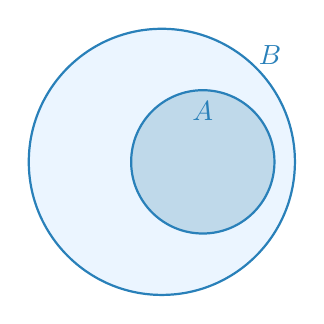
\begin{tikzpicture}[scale=1.3]
        \fill[boxBlueBg] (0,0) circle (1.3);
        \fill[boxBlue!30] (0.4,0) circle (0.7);
        \draw[boxBlue, thick] (0,0) circle (1.3) node[above right=1.1cm] {$B$};
        \draw[boxBlue, thick] (0.4,0) circle (0.7) node[above=0.4cm] {$A$};
      \end{tikzpicture}

    \column{0.45\textwidth}
      \centering
      \textbf{$A \not\subseteq B$}

      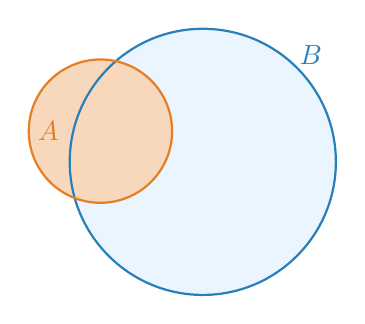
\begin{tikzpicture}[scale=1.3]
        \fill[boxBlueBg] (0,0) circle (1.3);
        \fill[boxOrange!30] (-1,0.3) circle (0.7);
        \draw[boxBlue, thick] (0,0) circle (1.3) node[above right=1.1cm] {$B$};
        \draw[boxOrange, thick] (-1,0.3) circle (0.7) node[left=0.4cm] {$A$};
      \end{tikzpicture}
  \end{columns}
\end{frame}

\begin{frame}{เซตกำลัง (Power Set)}
  \begin{explanation}[นิยาม]
    \textbf{เซตกำลัง} ของ $A$ ($P(A)$) คือ \highlight{เซตของสับเซตทั้งหมด} ของ $A$

    \medskip
    $P(A) = \{X \mid X \subseteq A\}$

    \medskip
    \textbf{จำนวนสมาชิก:} $|P(A)| = 2^{|A|}$
  \end{explanation}

  \begin{exambox}[ตัวอย่าง]
    ถ้า $A = \{1, 2\}$ แล้ว

    \medskip
    $P(A) = \bigl\{\emptyset, \{1\}, \{2\}, \{1, 2\}\bigr\}$

    \medskip
    $|P(A)| = 2^{2} = 4$ \quad (มีสมาชิก 4 ตัว)
  \end{exambox}
\end{frame}

\subsection{ช่วงของจำนวนจริง (Intervals)}

\begin{frame}{ช่วง (Intervals) — สับเซตของ $\R$}
  \begin{explanation}[นิยาม]
    \textbf{ช่วง (Interval)} คือสับเซตของจำนวนจริงที่ประกอบด้วยจำนวนจริงทุกจำนวน
    ที่อยู่ระหว่างค่าที่กำหนดสองค่า การเขียนช่วงใช้เครื่องหมายวงเล็บดังนี้:

    \medskip
    \begin{itemize}
      \item $[$ หรือ $]$ = \highlight{รวมจุดปลาย} (closed) — ใช้กับ $\leq$ หรือ $\geq$
      \item $($ หรือ $)$ = \highlight{ไม่รวมจุดปลาย} (open) — ใช้กับ $<$ หรือ $>$
    \end{itemize}
  \end{explanation}

  \begin{columns}[T]
    \column{0.5\textwidth}
      \textbf{ช่วงจำกัด (Bounded Intervals)}

      $[1, 2] = \{x \in \R \mid 1 \leq x \leq 2\}$

      $[1, 2) = \{x \in \R \mid 1 \leq x < 2\}$

      $(1, 2] = \{x \in \R \mid 1 < x \leq 2\}$

      $(1, 2) = \{x \in \R \mid 1 < x < 2\}$

    \column{0.5\textwidth}
      \textbf{ช่วงอนันต์ (Unbounded Intervals)}

      $[1, \infty) = \{x \in \R \mid x \geq 1\}$

      $(1, \infty) = \{x \in \R \mid x > 1\}$

      $(-\infty, 5] = \{x \in \R \mid x \leq 5\}$

      $(-\infty, 5) = \{x \in \R \mid x < 5\}$

      $(-\infty, \infty) = \R$
  \end{columns}
\end{frame}

\begin{frame}{ตัวอย่าง: การเขียนช่วง}
  \begin{exambox}[ตัวอย่างการเขียนช่วงแบบต่าง ๆ]
    \begin{enumerate}
      \item \textbf{ช่วง $[1, 2)$} — จำนวนจริงตั้งแต่ 1 ถึง 2
        \begin{itemize}
          \item $1 \in [1, 2)$ เพราะ $1 \geq 1$ (รวมจุดปลายซ้าย)
          \item $2 \notin [1, 2)$ เพราะ $2 \not< 2$ (ไม่รวมจุดปลายขวา)
          \item $1.5 \in [1, 2)$ เพราะ $1 \leq 1.5 < 2$
        \end{itemize}

      \item \textbf{ช่วง $(-\infty, 5]$} — จำนวนจริงทั้งหมดที่ $\leq 5$
        \begin{itemize}
          \item $5 \in (-\infty, 5]$, \quad $0 \in (-\infty, 5]$, \quad $-100 \in (-\infty, 5]$
          \item $6 \notin (-\infty, 5]$ เพราะ $6 > 5$
        \end{itemize}

      \item \textbf{ช่วง $(1, \infty)$} — จำนวนจริงทั้งหมดที่ $> 1$
        \begin{itemize}
          \item $2 \in (1, \infty)$, \quad $100 \in (1, \infty)$
          \item $1 \notin (1, \infty)$ เพราะต้องมากกว่า 1 อย่างเดียว (ไม่รวม 1)
        \end{itemize}
    \end{enumerate}
  \end{exambox}
\end{frame}

% ===========================================================================
%  SECTION 2: การดำเนินการของเซต (Set Operations)
% ===========================================================================
\section{การดำเนินการของเซต (Set Operations)}

\subsection{ยูเนียน อินเตอร์เซกชัน และคอมพลีเมนต์}

\begin{frame}{ยูเนียน (Union)}
  \begin{explanation}[นิยาม]
    \textbf{ยูเนียน} ของ $A$ และ $B$ ($A \cup B$) คือเซตของสมาชิกที่อยู่ใน $A$ \highlight{หรือ} อยู่ใน $B$ (หรือทั้งคู่)

    \medskip
    $A \cup B = \{x \mid x \in A \text{ หรือ } x \in B\}$
  \end{explanation}

  \begin{columns}[T]
    \column{0.45\textwidth}
      \centering
      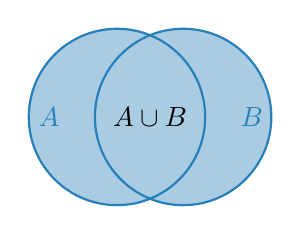
\begin{tikzpicture}[scale=1.4]
        \fill[boxBlue!40] (-0.3,0) circle (0.8);
        \fill[boxBlue!40] (0.3,0) circle (0.8);
        \draw[boxBlue, thick] (-0.3,0) circle (0.8) node[left=0.6cm] {$A$};
        \draw[boxBlue, thick] (0.3,0) circle (0.8) node[right=0.6cm] {$B$};
        \node at (0,0) {$A \cup B$};
      \end{tikzpicture}

    \column{0.45\textwidth}
      \begin{exambox}[ตัวอย่าง]
        $A = \{1, 2, 3\}$ \\
        $B = \{3, 4, 5\}$

        \medskip
        $A \cup B = \{1, 2, 3, 4, 5\}$
      \end{exambox}
  \end{columns}
\end{frame}

\begin{frame}{อินเตอร์เซกชัน (Intersection)}
  \begin{explanation}[นิยาม]
    \textbf{อินเตอร์เซกชัน} ของ $A$ และ $B$ ($A \cap B$) คือเซตของสมาชิกที่อยู่ใน $A$ \highlight{และ} อยู่ใน $B$

    \medskip
    $A \cap B = \{x \mid x \in A \text{ และ } x \in B\}$
  \end{explanation}

  \begin{columns}[T]
    \column{0.45\textwidth}
      \centering
      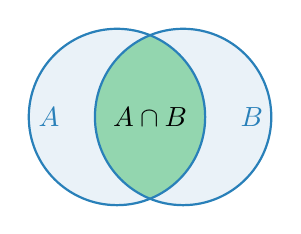
\begin{tikzpicture}[scale=1.4]
        \fill[boxBlue!10] (-0.3,0) circle (0.8);
        \fill[boxBlue!10] (0.3,0) circle (0.8);
        \begin{scope}
          \clip (-0.3,0) circle (0.8);
          \fill[boxGreen!50] (0.3,0) circle (0.8);
        \end{scope}
        \draw[boxBlue, thick] (-0.3,0) circle (0.8) node[left=0.6cm] {$A$};
        \draw[boxBlue, thick] (0.3,0) circle (0.8) node[right=0.6cm] {$B$};
        \node at (0,0) {$A \cap B$};
      \end{tikzpicture}

    \column{0.45\textwidth}
      \begin{exambox}[ตัวอย่าง]
        $A = \{1, 2, 3\}$ \\
        $B = \{3, 4, 5\}$

        \medskip
        $A \cap B = \{3\}$
      \end{exambox}
  \end{columns}
\end{frame}

\begin{frame}{คอมพลีเมนต์ (Complement)}
  \begin{explanation}[นิยาม]
    \textbf{คอมพลีเมนต์} ของ $A$ ($A'$ หรือ $A^c$ หรือ $\overline{A}$) คือเซตของสมาชิกใน $U$
    ที่ \highlight{ไม่อยู่ใน} $A$

    \medskip
    $A' = \{x \in U \mid x \notin A\}$
  \end{explanation}

  \begin{columns}[T]
    \column{0.45\textwidth}
      \centering
      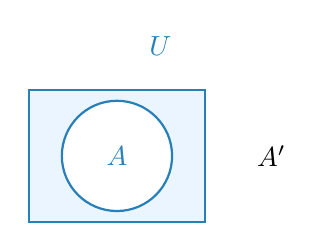
\begin{tikzpicture}[scale=1.4]
        \fill[boxBlueBg] (-0.8,-0.6) rectangle (0.8,0.6);
        \fill[white] (0,0) circle (0.5);
        \draw[boxBlue, thick] (-0.8,-0.6) rectangle (0.8,0.6) node[above left=0.3cm] {$U$};
        \draw[boxBlue, thick] (0,0) circle (0.5) node {$A$};
        \node at (1.4,0) {$A'$};
      \end{tikzpicture}

    \column{0.45\textwidth}
      \begin{exambox}[ตัวอย่าง]
        $U = \{1, 2, 3, 4, 5\}$ \\
        $A = \{1, 2\}$

        \medskip
        $A' = \{3, 4, 5\}$
      \end{exambox}
  \end{columns}
\end{frame}

\begin{frame}{ผลต่างของเซต (Set Difference)}
  \begin{explanation}[นิยาม]
    \textbf{ผลต่าง} $A - B$ (หรือ $A \setminus B$) คือเซตของสมาชิกที่อยู่ใน $A$ แต่ \highlight{ไม่อยู่ใน} $B$

    \medskip
    $A - B = \{x \mid x \in A \text{ และ } x \notin B\}$
  \end{explanation}

  \begin{exambox}[ตัวอย่าง]
    $A = \{1, 2, 3, 4\}$, \quad $B = \{3, 4, 5, 6\}$

    \medskip
    $A - B = \{1, 2\}$ \quad (สมาชิกที่อยู่ใน $A$ แต่ไม่อยู่ใน $B$)

    $B - A = \{5, 6\}$ \quad (สมาชิกที่อยู่ใน $B$ แต่ไม่อยู่ใน $A$)

    \medskip
    \textbf{สังเกต:} $A - B \neq B - A$ (โดยทั่วไป)
  \end{exambox}
\end{frame}

% ===========================================================================
%  SECTION 3: กฎทางพีชคณิตของเซต (Laws of Set Algebra)
% ===========================================================================
\section{กฎทางพีชคณิตของเซต (Laws of Set Algebra)}

\subsection{สมบัติพื้นฐาน}

\begin{frame}{สมบัติการสลับที่และการเปลี่ยนหมู่}
  \begin{explanation}[สมบัติการสลับที่ (Commutative Laws)]
    \begin{enumerate}
      \item $A \cup B = B \cup A$
      \item $A \cap B = B \cap A$
    \end{enumerate}
  \end{explanation}

  \begin{explanation}[สมบัติการเปลี่ยนหมู่ (Associative Laws)]
    \begin{enumerate}
      \item $(A \cup B) \cup C = A \cup (B \cup C)$
      \item $(A \cap B) \cap C = A \cap (B \cap C)$
    \end{enumerate}
  \end{explanation}

  \begin{intuition}[จำง่าย ๆ]
    \begin{itemize}
      \item \textbf{สลับที่} = สลับลำดับแล้วผลลัพธ์เหมือนเดิม (เหมือน $a+b = b+a$)
      \item \textbf{เปลี่ยนหมู่} = จัดกลุ่มใหม่แล้วผลลัพธ์เหมือนเดิม (เหมือน $(a+b)+c = a+(b+c)$)
    \end{itemize}
  \end{intuition}
\end{frame}

\begin{frame}{สมบัติการแจกแจงและนิจพล}
  \begin{explanation}[สมบัติการแจกแจง (Distributive Laws)]
    \begin{enumerate}
      \item $A \cup (B \cap C) = (A \cup B) \cap (A \cup C)$
      \item $A \cap (B \cup C) = (A \cap B) \cup (A \cap C)$
    \end{enumerate}
  \end{explanation}

  \begin{explanation}[สมบัตินิจพล (Identity Laws)]
    \begin{enumerate}
      \item $A \cup \emptyset = A$
      \item $A \cap U = A$
      \item $A \cup U = U$
      \item $A \cap \emptyset = \emptyset$
    \end{enumerate}
  \end{explanation}
\end{frame}

\subsection{กฎเดอมอร์แกน (De Morgan's Laws)}

\begin{frame}{กฎเดอมอร์แกน (De Morgan's Laws)}
  \begin{explanation}[กฎเดอมอร์แกน — สำคัญมาก!]
    \begin{enumerate}
      \item \highlight{$(A \cup B)' = A' \cap B'$}
      \item \highlight{$(A \cap B)' = A' \cup B'$}
    \end{enumerate}
  \end{explanation}

  \begin{intuition}[วิธีจำ]
    \textbf{กระจายนิเสธเข้าไป แล้วกลับเครื่องหมาย:}
    $\cup$ กลายเป็น $\cap$, \quad $\cap$ กลายเป็น $\cup$

    เหมือนกับ $\lnot(p \lor q) \equiv \lnot p \land \lnot q$ ในตรรกศาสตร์!
  \end{intuition}
\end{frame}

\begin{frame}{ตัวอย่าง: กฎเดอมอร์แกน}
  \begin{exambox}[ตรวจสอบ]
    $U = \{1, 2, 3, 4, 5\}$, \quad $A = \{1, 2\}$, \quad $B = \{2, 3\}$

    \medskip
    $A \cup B = \{1, 2, 3\}$ \quad $\Rightarrow$ \quad $(A \cup B)' = \{4, 5\}$

    $A' = \{3, 4, 5\}$, \; $B' = \{1, 4, 5\}$ \quad $\Rightarrow$ \quad $A' \cap B' = \{4, 5\}$

    \medskip
    ดังนั้น $(A \cup B)' = A' \cap B'$ \quad $\checkmark$
  \end{exambox}
\end{frame}

\begin{frame}{กฎอื่น ๆ ที่สำคัญ}
  \begin{explanation}[Complement Laws]
    \begin{enumerate}
      \item $A \cup A' = U$
      \item $A \cap A' = \emptyset$
      \item $(A')' = A$
      \item $\emptyset' = U$, \quad $U' = \emptyset$
    \end{enumerate}
  \end{explanation}
\end{frame}

\begin{frame}{กฎอื่น ๆ (ต่อ)}
  \begin{explanation}[Idempotent Laws]
    \begin{enumerate}
      \item $A \cup A = A$
      \item $A \cap A = A$
    \end{enumerate}
  \end{explanation}

  \begin{explanation}[Absorption Laws (การดูดซึม)]
    \begin{enumerate}
      \item $A \cup (A \cap B) = A$
      \item $A \cap (A \cup B) = A$
    \end{enumerate}
  \end{explanation}

  \begin{intuition}[Absorption = การดูดซึม]
    $A$ ``ดูดซึม'' $B$ เข้าไป — ถ้า $A$ อยู่แล้ว ไม่ว่าจะ $\cup$ หรือ $\cap$ กับ $B$
    ผลลัพธ์ก็ยังเป็น $A$ (เมื่อ $B$ ถูกดูดซึมโดย $A$)
  \end{intuition}
\end{frame}

% ===========================================================================
%  SECTION 4: ผลคูณคาร์ทีเซียน (Cartesian Product)
% ===========================================================================
\section{ผลคูณคาร์ทีเซียน (Cartesian Product)}

\begin{frame}{ผลคูณคาร์ทีเซียน}
  \begin{explanation}[นิยาม]
    \textbf{ผลคูณคาร์ทีเซียน} ของ $A$ และ $B$ ($A \times B$) คือเซตของคู่อันดับ $(a, b)$ ทั้งหมด
    โดยที่ $a \in A$ และ $b \in B$

    \medskip
    $A \times B = \{(a, b) \mid a \in A \text{ และ } b \in B\}$

    \medskip
    \textbf{จำนวนสมาชิก:} $|A \times B| = |A| \times |B|$
  \end{explanation}

  \begin{exambox}[ตัวอย่าง]
    $A = \{1, 2\}$, \quad $B = \{x, y\}$

    \medskip
    $A \times B = \{(1, x), (1, y), (2, x), (2, y)\}$

    \medskip
    \textbf{สังเกต:} $A \times B \neq B \times A$ โดยทั่วไป (ลำดับสำคัญ)
  \end{exambox}
\end{frame}

% ===========================================================================
%  SECTION 5: หลักการเพิ่มเข้าและตัดออก (Inclusion-Exclusion)
% ===========================================================================
\section{หลักการเพิ่มเข้าและตัดออก (Inclusion-Exclusion)}

\begin{frame}{จำนวนสมาชิกของยูเนียน}
  \begin{explanation}[หลักการเพิ่มเข้าและตัดออก สำหรับ 2 เซต]
    \[
      |A \cup B| = |A| + |B| - |A \cap B|
    \]
  \end{explanation}

  \begin{center}
    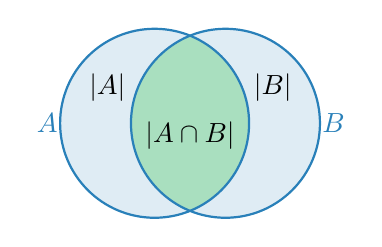
\begin{tikzpicture}[scale=1.5]
      \fill[boxBlue!15] (-0.3,0) circle (0.8);
      \fill[boxBlue!15] (0.3,0) circle (0.8);
      \begin{scope}
        \clip (-0.3,0) circle (0.8);
        \fill[boxGreen!40] (0.3,0) circle (0.8);
      \end{scope}
      \draw[boxBlue, thick] (-0.3,0) circle (0.8) node[left=1.1cm] {$A$};
      \draw[boxBlue, thick] (0.3,0) circle (0.8) node[right=1.1cm] {$B$};

      \node at (-0.7,0.3) {$|A|$};
      \node at (0.7,0.3) {$|B|$};
      \node at (0,-0.1) {$|A \cap B|$};
    \end{tikzpicture}
  \end{center}

  \begin{intuition}[เหตุผล]
    เมื่อบวก $|A| + |B|$ สมาชิกใน $A \cap B$ ถูกนับ \highlight{ซ้ำ 2 ครั้ง}
    จึงต้องลบออก 1 ครั้ง
  \end{intuition}
\end{frame}

\begin{frame}{ตัวอย่าง: Inclusion-Exclusion}
  \begin{exambox}[โจทย์]
    ในการสำรวจนักเรียน 100 คน พบว่าชอบคณิตศาสตร์ 60 คน
    ชอบคอมพิวเตอร์ 45 คน และชอบทั้งสองวิชา 20 คน
    จงหาจำนวนนักเรียนที่
    \begin{enumerate}
      \item[(ก)] ชอบคณิตศาสตร์หรือคอมพิวเตอร์
      \item[(ข)] ไม่ชอบทั้งสองวิชา
    \end{enumerate}
  \end{exambox}

  \begin{solbox}[วิธีทำ]
    ให้ $M$ = ชอบคณิตศาสตร์, $C$ = ชอบคอมพิวเตอร์

    $|M| = 60$, $|C| = 45$, $|M \cap C| = 20$

    (ก) $|M \cup C| = 60 + 45 - 20 = 85$ คน

    (ข) ไม่ชอบทั้งสอง = ทั้งหมด - ชอบอย่างน้อยหนึ่ง
    $= 100 - 85 = 15$ คน
  \end{solbox}
\end{frame}

\begin{frame}{Inclusion-Exclusion สำหรับ 3 เซต}
  \begin{explanation}[สูตรสำหรับ 3 เซต]
    \[
      |A \cup B \cup C| = |A| + |B| + |C|
      - |A \cap B| - |A \cap C| - |B \cap C|
      + |A \cap B \cap C|
    \]
  \end{explanation}

  \begin{intuition}[หลักการ]
    \begin{itemize}
      \item \highlight{บวก} สมาชิกของ 1 เซต ($|A|+|B|+|C|$)
      \item \highlight{ลบ} ส่วนที่ซ้ำกันของ 2 เซต ($-|A \cap B| - \ldots$)
      \item \highlight{บวกกลับ} ส่วนที่ซ้ำกันของ 3 เซต ($+|A \cap B \cap C|$)
    \end{itemize}
    หลักการ: \textbf{บวก-ลบ-บวก-ลบ สลับกันไป} ตามจำนวนเซตที่ซ้อนทับ
  \end{intuition}
\end{frame}

\begin{frame}{ตัวอย่าง: ข้อสอบจริง}
  \begin{exambox}[โจทย์ปี 67 ข้อ 13]
    กำหนดจำนวนสมาชิกในเซต $A, B, C$ และ $A \cup B$ เป็นดังนี้ $n(A)=6, n(B)=5, n(C)=4$ และ $n(A \cup B)=8$ เมื่อ $A \times B$ คือผลคูณคาร์ทีเซียนของ $A$ และ $B$ จงหา $n(A \times B) + n[(A \cap B) \times C] + n[(A-B) \times C]$
  \end{exambox}
  
  \begin{solbox}[วิธีทำ]
    $n(A \times B) = n(A) \times n(B) = 6 \times 5 = 30$ \newline
    $n(A \cap B) = n(A)+n(B)-n(A \cup B)=6+5-8=3$ \newline
    $n[(A \cap B) \times C] = n(A \cap B) \times n(C)=3\times 4=12$ \newline
    $n(A - B)=n(A)-n(A \cap B)=6-3=3$ \newline
    $n[(A-B) \times C]=n(A - B)\times n(C)=3\times 4=12$ \newline
    $n(A \times B) + n[(A \cap B) \times C] + n[(A-B) \times C]=30+12+12=54$
  \end{solbox}
\end{frame}

% ===========================================================================
%  SUMMARY
% ===========================================================================
\section{สรุป}

\begin{frame}{สรุปเนื้อหา}
  \begin{explanation}[สิ่งที่ได้เรียนรู้]
    \begin{enumerate}
      \item \textbf{เซต}: กลุ่มของสิ่งของ — เซตจำกัด vs เซตอนันต์
      \item \textbf{สับเซต \& เซตกำลัง}: $A \subseteq B$, $|P(A)| = 2^{|A|}$
      \item \textbf{การดำเนินการ}: $\cup$ (หรือ), $\cap$ (และ), $'$ (ไม่), $-$ (ผลต่าง), $\times$ (คาร์ทีเซียน)
      \item \textbf{กฎเดอมอร์แกน}: $(A \cup B)' = A' \cap B'$, \quad $(A \cap B)' = A' \cup B'$
      \item \textbf{Inclusion-Exclusion}: $|A \cup B| = |A| + |B| - |A \cap B|$
    \end{enumerate}
  \end{explanation}

  \begin{center}
    \large เอกสารนี้เป็นส่วนหนึ่งของเนื้อหาเตรียมสอบ \textbf{สอวน. คอมพิวเตอร์}
  \end{center}
\end{frame}

\end{document}
